

\tikzset{every picture/.style={line width=0.75pt}} %set default line width to 0.75pt        

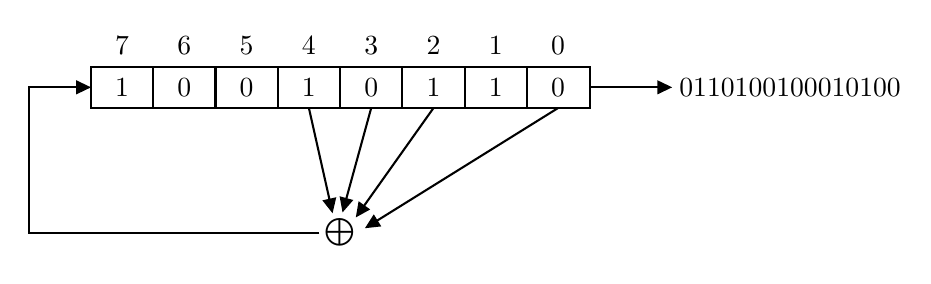
\begin{tikzpicture}[x=0.75pt,y=0.75pt,yscale=-1,xscale=1]
%uncomment if require: \path (0,120); %set diagram left start at 0, and has height of 120

%Shape: Rectangle [id:dp8699898407336639] 
\draw   (60,20) -- (300.4,20) -- (300.4,40) -- (60,40) -- cycle ;
%Straight Lines [id:da6480423944948943] 
\draw    (90,20) -- (90,40) ;
%Straight Lines [id:da1357097181943394] 
\draw    (120,20) -- (120,40) ;
%Straight Lines [id:da6348473634558065] 
\draw    (150,20) -- (150,40) ;
%Straight Lines [id:da9852363854962749] 
\draw    (180,19.97) -- (180,40) ;
%Straight Lines [id:da6251188632523177] 
\draw    (210,20) -- (210,40) ;
%Straight Lines [id:da9628068129583953] 
\draw    (240,20) -- (240,40) ;
%Straight Lines [id:da5093234988477329] 
\draw    (270,20) -- (270,40) ;
%Straight Lines [id:da506886279614565] 
\draw    (165,40) -- (175.74,87.74) ;
\draw [shift={(176.4,90.67)}, rotate = 257.32] [fill={rgb, 255:red, 0; green, 0; blue, 0 }  ][line width=0.08]  [draw opacity=0] (7.14,-3.43) -- (0,0) -- (7.14,3.43) -- cycle    ;
%Straight Lines [id:da08239608836085877] 
\draw    (195,40) -- (181.99,87.38) ;
\draw [shift={(181.2,90.27)}, rotate = 285.35] [fill={rgb, 255:red, 0; green, 0; blue, 0 }  ][line width=0.08]  [draw opacity=0] (7.14,-3.43) -- (0,0) -- (7.14,3.43) -- cycle    ;
%Straight Lines [id:da8508423498295425] 
\draw    (225,40) -- (189.34,90.22) ;
\draw [shift={(187.6,92.67)}, rotate = 305.38] [fill={rgb, 255:red, 0; green, 0; blue, 0 }  ][line width=0.08]  [draw opacity=0] (7.14,-3.43) -- (0,0) -- (7.14,3.43) -- cycle    ;
%Straight Lines [id:da1889764527983564] 
\draw    (285,40) -- (194.55,96.28) ;
\draw [shift={(192,97.87)}, rotate = 328.11] [fill={rgb, 255:red, 0; green, 0; blue, 0 }  ][line width=0.08]  [draw opacity=0] (7.14,-3.43) -- (0,0) -- (7.14,3.43) -- cycle    ;
%Straight Lines [id:da2853178114885824] 
\draw    (170,100) -- (30,100) -- (30,30) -- (57,30) ;
\draw [shift={(60,30)}, rotate = 180] [fill={rgb, 255:red, 0; green, 0; blue, 0 }  ][line width=0.08]  [draw opacity=0] (7.14,-3.43) -- (0,0) -- (7.14,3.43) -- cycle    ;
%Straight Lines [id:da8823488045232695] 
\draw    (300,30) -- (337,30) ;
\draw [shift={(340,30)}, rotate = 180] [fill={rgb, 255:red, 0; green, 0; blue, 0 }  ][line width=0.08]  [draw opacity=0] (7.14,-3.43) -- (0,0) -- (7.14,3.43) -- cycle    ;

% Text Node
\draw (75,30) node    {$1$};
% Text Node
\draw (105,29.97) node    {$0$};
% Text Node
\draw (135,30) node    {$0$};
% Text Node
\draw (165,30) node    {$1$};
% Text Node
\draw (195,30) node    {$0$};
% Text Node
\draw (225,30) node    {$1$};
% Text Node
\draw (255,30) node    {$1$};
% Text Node
\draw (285,30) node    {$0$};
% Text Node
\draw (75,10) node    {$7$};
% Text Node
\draw (105,10) node    {$6$};
% Text Node
\draw (135,10) node    {$5$};
% Text Node
\draw (165,10) node    {$4$};
% Text Node
\draw (195,10) node    {$3$};
% Text Node
\draw (225,10) node    {$2$};
% Text Node
\draw (255,10) node    {$1$};
% Text Node
\draw (285,10) node    {$0$};
% Text Node
\draw (180,100) node  [font=\large]  {$\bigoplus $};
% Text Node
\draw (342,30) node [anchor=west] [inner sep=0.75pt]    {$0110100100010100\dotsc $};


\end{tikzpicture}